\chapter{Einleitung}
\label{ch:intro}

\section{Motivation}
\label{sec:intro:motivation}
Viele Unternehmen verfügen über sensible Informationen, sei es zum Beispiel Versicherungen oder Krankenhäuser, die Telefonnummern und über Namen verfügen.
Diese Informationen werden auf gesicherten Servern gelagert, auf welche nur bestimmte Personen Berechtigungen haben.
Diese Personen verfügen über Profile, die ihnen diese Berechtigungen verfügen.
Jedoch kann es passieren, dass solche Profile gestohlen oder Personen gegeben werden, welche diese nicht haben sollten.
Berechtigungstrukturen sollen genau diese Szenarien verhindern.
Wird aber eine Berechtigungstruktur lange genutzt, werden nicht alle Richtlinien und Normen eingehalten, wodurch diese unsicherer und unübersichtlicher wird.
Das hat zur Folge, dass das Risiko, dass die sensitiven Informationen in nicht autorisierten Hände kommt, steigt.
Dadürch können nämlich "`Super Accounts"' entstehen.
"`Super Accounts"' verfügen über zu viele bis zu gar allen Berechtigungen im System.
Sollte diese Person durch einen Angriff diesen "`Super Account"' verlieren, wäre die gesamte Struktur kompromitiert.
Dasselbe ist der Fall, wenn ein Mitarbeiter mit einem solchen Account dem Unternehmen schaden will.

\begin{figure}[h!]
 \centering
 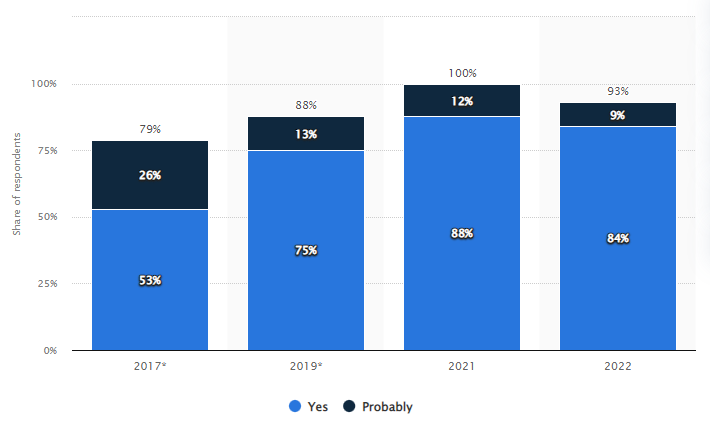
\includegraphics[width=1\textwidth]{gfx/Picture/Cyber_Crime.PNG}
 \caption{Eine Umfrage von Deutschen Unternehmen, die von Daten Diebstahl, Espionage oder Sabotage betroffen waren.\cite{Stat22}}
 \label{fig:Crime}
\end{figure}

Wie man in der Grafik (\ref{fig:Crime}) erkennen kann, waren 88\% der befragten Unternehmen in Deutschland von Daten Diebstahl, Espionage oder Sabotage in 2021 betroffen.
In 2022 liegt die Zahl bei 84\%.
Wobei man berücksichtigen muss, dass diese Befragung zwischen Januar and März statt gefunden und dies daher nur das erste Quartal von 2022 abdeckt.
Aufgrund dessen, dass solche Angriffe wahrscheinlich sind, darf es keine "`Super Accounts"' geben, da diese ansonsten in solchen Angriffen als Schwachstelle ausgenutzt werden können.

%
% Section: Ziele
%
\section{Ziel der Arbeit}
\label{sec:intro:goal}
Ei choro aeterno antiopam mea, ut eos erant homero concludaturque. Albucius appellantur deterruisset id eam, vivendum partiendo dissentiet ei ius. Vis melius facilisis ea, sea id convenire referrentur, takimata adolescens ex duo. Ei harum argumentum per. Eam vidit exerci appetere ad, ut vel zzril intellegam interpretaris.

Errem omnium ea per, pro \ac{UML} congue populo ornatus cu, ex qui dicant nemore melius. No pri diam iriure euismod. Graecis eleifend appellantur quo id. Id corpora inimicus nam, facer nonummy ne pro, kasd repudiandae ei mei. Mea menandri mediocrem dissentiet cu, ex nominati imperdiet nec, sea odio duis vocent ei. Tempor everti appareat cu ius, ridens audiam an qui, aliquid admodum conceptam ne qui. Vis ea melius nostrum, mel alienum ac elit id nibh pretium pulvina euripidis eu.

Ei choro aeterno antiopam mea, labitur bonorum pri no. His no decore nemore graecis. In eos meis nominavi, liber soluta vim cu. Integer consectetur, mi congue feugiat rhoncus, ante libero consectetur eros, et interdum nulla velit non velit. Mauris pharetra venenatis porttitor. Suspendisse et risus at dui gravida hendrerit. Aenean auctor interdum sodales. Etiam tortor orci, scelerisque in gravida eu, varius a massa. Ut sem odio, commodo id pharetra eu, dictum vitae. 

%
% Section: Struktur der Arbeit
%
\section{Gliederung}
\label{sec:intro:structure}
Nulla fastidii ea ius, exerci suscipit instructior te nam, in ullum postulant quo. Congue quaestio philosophia his at, sea odio autem vulputate ex. Cu usu mucius iisque voluptua. Sit maiorum propriae at, ea cum \ac{API} primis intellegat. Hinc cotidieque reprehendunt eu nec. Autem timeam deleniti usu id, in nec nibh altera.
